\documentclass{llncs}

\usepackage{hyperref}
\usepackage{graphicx}
\usepackage{epstopdf}
\usepackage{listings}
\usepackage{caption}
\usepackage[dvipsnames]{xcolor}
\usepackage{float}
\usepackage{geometry}\geometry{
 a4paper,
 left=8em,
 right=8em
}

\renewcommand{\lstlistingname}{Code}

\newcommand\realnumberstyle[1]{}

\makeatletter
\newcommand{\zebra}[3]{%
	{\realnumberstyle{#3}}%
   	\begingroup
    	\ifodd\value{lstnumber}%
        	\color{#1}%
    	\else
        	\color{#2}%
    	\fi
    	\ifnum\value{lstnumber} > 9
        	\rlap{\hspace*{\lst@numbersep}\hspace*{0.6em}%
        	\color@block{\linewidth}{\ht\strutbox}{\dp\strutbox}%
        	}%
    	\else
        	\rlap{\hspace*{\lst@numbersep}\hspace*{0.1em}%
        	\color@block{\linewidth}{\ht\strutbox}{\dp\strutbox}%
        	}%
    	\fi
    \endgroup
}
\makeatother

\makeatletter
\newcommand{\code}[1]{%
	\texttt{#1}%
	\fontdimen2\font=0.4em
	\fontdimen3\font=0.2em
	\fontdimen4\font=0.1em
	\fontdimen7\font=0.1em
	\hyphenchar\font=`\-
}
\makeatother

\lstset{
	numbersep=10pt,
	breaklines=true,
	showstringspaces=false,
	breakatwhitespace=true,
	frame=b,
	framexleftmargin=15pt,
  	framexbottommargin=15pt,
  	framextopmargin=15pt,
	xleftmargin=\parindent,
	showstringspaces=false,
	basicstyle=\footnotesize\ttfamily,
	numberstyle=\zebra{gray!50}{gray!10}{}\tiny,
	keywordstyle=\color{red},
	commentstyle=\color{OliveGreen},
	captionpos=b,
}

\DeclareCaptionFormat{listing}{#1#2#3}
\captionsetup[lstlisting]{%
	format=listing,
	singlelinecheck=false,
	margin=0pt,
	labelfont=bf
}
\captionsetup[figure]{%
	format=listing,
	singlelinecheck=false,
	margin=0pt,
	labelfont=bf,
}

\begin{document}
\title{Time Synchronization II}

%If you're using runningheads you can add an abreviated title for the running head on odd pages using the following
%\titlerunning{abreviated title goes here}
%and an alternative title for the table of contents:
%\toctitle{table of contents title}

\subtitle{Rate-Based Synchronous Diffusion}

%For a single author
%\author{Author Name}

%For multiple authors:
\author{Pascal Gadient\\ Domenico Iapello \\ Felix Langenegger} 


%If using runnningheads you can abbreviate the author name on even pages:
%\authorrunning{abbreviated author name}
%and you can change the author name in the table of contents
%\tocauthor{enhanced author name}

%For a single institute
%\institute{Institute Name \email{email address}}

% If authors are from different institutes 
\institute{University of Bern \\ Communication and Distributed Systems }

%to remove your email just remove '\email{email address}'
% you can also remove the thanks footnote by removing '\thanks{Thank you to...}'


\maketitle

%\begin{abstract}
%abstract text goes here - Lorem ipsum dolor sit amet, consectetur adipiscing elit, sed do eiusmod tempor incididunt ut labore et dolore magna aliqua.
%\end{abstract}

\section{Protocol Introduction}
% Maximum 1 page about the theoretical basics of the experiment.
A sensor network is basically made of some sensor nodes that are linked together. To fulfil the main goals of the sensor network the time synchronisation of the network nodes is important.  For example, it is useful to have the same time frames on each node to compare the measurements of each node. Or if the network is a mobile sensor network, the exact localisation of each node could be demanded, which can only be provided, if the nodes have synchronised time. Additionally, the management of the duty cycles can only be meaningful if the nodes are in sync.\\
The requirements of an accurate time synchronisation algorithm are amongst others, precision, energy efficiency, a small memory footprint, scalability and robustness. It should be obvious that the time should be as exact as possible on every node. Therefore, the algorithm should be as efficient as possible because of the limited energy resources. Most of all, the time synchronisation is not the main application of the node itself, so the algorithm should not consume most of the resources as computing time and energy. The same goes for the memory.
\noindent The time synchronisation algorithm should be scalable in two dimensions. Firstly, it has to be scalable on each device, that means it should run on nodes with very small resources. Secondly, it should be scalable for a lot of devices in a sensor network, that means as more and more nodes are added to the network, the algorithm should run as robust as possible.\\
\noindent This project report explains how we solved the problem of time synchronisation base on the Rate Based Synchronous Diffusion Algorithm (RBSDA)\footnote{See lecture slide: V. Time Synchronization - 3.3.1 Diffusion-based Synchronization p. 29-30. This slides are based on the paper: Global Clock Synchronization
in Sensor Networks by Qun Li and  Daniela Rus\cite{LiRus2006}}. The basic idea of the RBSDA is to know all the visible nodes of one specific node and then to iterate over the known neighbours to determine the time offset via round-trip synchronisation.\\
In the Methods section we explain how we implemented this algorithm to achieve the synchronisation. Then we expose how our experimental setup looked like. In the section Measurement Procedure we show how we obtained the measurements. The results we got we  illustrate in the next paragraph. And finally we reveal some concluding thoughts about our work. 

\section{Methods}
%Especially, describe the methods used to realize the protocol (functions in the code and their functionality)

First, we will speak in detail about the synchronisation algorithm itself and discuss how it works. Later, we pin-point some programming specialities of the used sensor nodes and finally, we present some debugging habits and methods used to ensure a fully functional implementation.
\bigbreak
\noindent The synchronisation algorithm progresses in three steps: Initially, the sensor nodes generates an internal representation of the surrounding neighbour nodes. Afterwards, it sends round-trip-time (RTT) request packets to all discovered nodes and stores then each node's received RTT together with the remote timestamp into the previously created neighbour node table representation. Finally, we calculate the median of all skews with respect to the RTTs and adjust therefore the local node time with these results multiplied by a constant factor alpha. We repeat the steps starting with the RTT request as long as we try to stay in sync with the other nodes (in general this is equivalent to the node's lifetime). This process is described in detail at code \ref{lst:algo}.

\begin{lstlisting}%
	[language=C, numbers=left, caption={Diffusion algorithm (DA) used to synchronise the whole sensor network}, label={lst:algo}]
// Do the following with some given frequency
  for each sensor n_i in the network do
    Exchange clock times with n_iís neighbours
      for each neighbour n_j do
        Let the time difference between n_i and n_j be t_i - t_j
          Change n_iís time to t_i - r_ij (t_i - t_j)
\end{lstlisting}

\noindent On a high-level perspective this converges, because each node adjusts itself towards the time of its neighbours. Hence, the more neighbours are seeing each other, the faster the synchronisation time in network converges. However, if there are some partition-like structures in the network it will still converge, but we will encounter disproportionately long synchronisation sequences. This is a result of a few nodes that form a bridge between two different time clusters, so all time adjustments between both clusters will involve these few nodes. Thus, the impact on the whole network is proportionally small, caused by the median calculations (a big skew divided by the amount of (many) nodes results in a small correction value). Last, but not least, the alpha value only guarantees a convergence while being in the range (0, 1). Hence, with a value of one, the time would oscillate back and forth and as an outcome it wouldn't converge at all. The same goes for an alpha value set to zero. With this constraint, no adjustments would take place at all (skew adjustment would always be zero in this scenario).
\bigbreak
\noindent A side mark for the RTT calculations: We consider only half the RTT, because the time set by the remote node travels only from the remote node to the corresponding node, i. e. half of the RTT time is used.\\
Now, we will have a look at some code that handles the skew adjustment in the DA-algorithm at code \ref{lst:code}.

\begin{lstlisting}%
	[language=C, numbers=left, caption={Skew Adjustment},label={lst:code}]
static void updateMyTime() {
  totalClockSkew = 0;
  activeNeighbourCount = 0;
  for (i5 = 0; i5 < MAX_NEIGHBOURS; i5++) {
    if (neighbours[i5].activeState) {
      activeNeighbourCount += 1;
      totalClockSkew += neighbours[i5].skew / ALPHA;
      neighbours[i5].skew = 0;
      neighbours[i5].rtt = 0;
      neighbours[i5].activeState = 0;
    }
  }

  if (activeNeighbourCount > 0) {
    totalClockSkew = totalClockSkew / activeNeighbourCount;
    clockCorrection = clock_time() + totalClockSkew;
    clock_set(clockCorrection, clockCorrection);
  }
}
\end{lstlisting}
\noindent In the code above we can easily see several specialities that occur in general on embedded devices such as our used sensors:
\begin{enumerate}
\item Floating-point unit does not exist, hence, we have to use divisions instead of floating-point multiplications (as shown in line 7).
\item Most hardware-specific system calls are not that well documented, we assume this is an outcome of embedded CPU designers, that set the focus on the chip, rather than the diverse operating systems that drive the chip. (As shown in line 17)
\item C code is used in general, as a result of the small memory and CPU footprint requirement.
\end{enumerate}

\noindent While contributing to this project, we were in need of many different debugging strategies, because C programming can be very painful, especially for team members that aren't that experienced with low-level programming.
So we developed strategies that can be roughly assigned to one of these two classes: Syntax-Supporting Strategies (SSS), as well as Logic-Supporting Strategies (LSS). 
A prime example of the SSS is the separately maintained "Playground.c" file in which we performed sandbox runs of some complicated code blocks, that upon successful validation eventually got in the main code base.
In contrast the LSS consist of mainly three approaches:
\begin{enumerate}
\item Simplify the code as much as possible (i.e. using structs for message exchanges and internal data representations and trying to reduce code complexity in general).
\item Analysis and verification of the generated logs.
\item Creation of decision-trees for sophisticated code blocks.
\end{enumerate}
% TODO: Uebgergang
Booting up a node results in loading two network protocol stacks, technically speaking, the unicast and the broadcast message handlers. Whilst the broadcast module disseminates the node's id along the neighbour nodes within the main program loop, the broadcast receiver block \code{recv\_bc(...)} recognises these messages and stores the corresponding neighbour in the node's neighbour table with \code{addNeighbour(unsigned short id)}. Further in the main loop the code requests RTTs via unicast messages from all neighbours stored in the neighbour table with \code{requestRTT(unsigned short id)}. As soon as they get replied, the \code{recv\_uc(...)} callback method extends the neighbour list with the received data via \code{saveRTT(unsigned short id, unsigned short rtt, signed long skew)}.
After polling each neighbour, the own time gets adjusted by \code{updateMyTime()}. Accordingly, the saved RTT and skew data gets deleted and the process repeats again within the main program loop.
Some more casual methods can be found in the code as well. For example there exist some led enabler and disabler methods with the corresponding callbacks (\code{enableLED(int color), disableLED(int color)}), as well as print methods for additional debugging \code{print\-Neighbor\-List()}), or the \code{calcTimeDifference(unsigned short actualTimeOwn, un\-sign\-ed short rttCorrTimeOther)} method used to calculate the time difference based on the time of two nodes with respect to tick overflows.

\section{Experimental Setup}

For the lecture `Sensor Network and Internet of things' each member got two sensor nodes called Telosb which were assembled by Crossbow\footnote{The datasheet for the node can be found on: \url{http://www.willow.co.uk/TelosB_Datasheet.pdf}}. The nodes run an operating system called Contiki\footnote{TODO: more infos to add}.\\
The assignment for the project was divided into two iterations. The first phase was to implement a prototype of the algorithm, which we planned to run on four of our nodes. In the second phase we had to adapt the software, so that it can run on the TARWIS\footnote{TODO. Reference} network with up to 40 nodes.

%\subsection{Prototype}

%\subsection{TRAWIS}

\section{Measurement Procedure}
In the beginning we inspected carefully each print statement in the console, but as further we came, the less feasible it got. Hence, we began to write parsers for different purposes which can in combination with some gnuplot\footnote{TODO: Reference} scripts nicely visualise the outcome of the synchronisation process. The endproducts of these parsers and scripts are shown as figures in the next few sections.

\section{Results and Analysis}

In this section we present some gathered results from our experiments, as well as some additional explanations and interpretations. The experiments consists of as less as four nodes in local execution and scales between 10 up to 40 nodes for the testbed runs. We run the experiment locally and on TARWIS with these three different configurations:
\begin{enumerate}
\item Normal run
\item Fast run
\item Fast run with some node resets after 60 min
\end{enumerate}
We performed additional measurements with different alpha values apart from the previously mentioned three setups.\\
Important side mark for TARWIS results: It lies in the nature of a heavily used, commonly shared testbed at a remote location that the results are not every time perfectly deterministic. This may be caused by accidentally performed system maintenance on-site, other users that are requesting much capacity at that same time, or workload that uses some shared resources on the specific cluster. Therefore, we had to use larger timeouts and intervals on TARWIS as with the local setup to obtain valid results.
\begin{figure}[H]
	\centering
	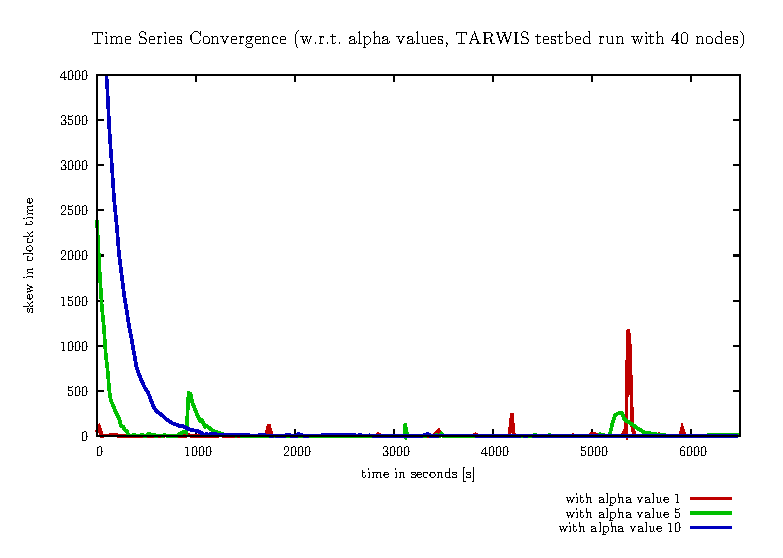
\includegraphics[scale=0.8]{images/FIG_01.eps}
	\caption{Time series convergence with respect to alpha values}
	\label{fig:alpha}
\end{figure}

\noindent In figure \ref{fig:alpha} we can clearly see that the algorithm is able to reach convergence around 250 seconds with a default alpha value of 5. The small amplitudes in the figure are non-deterministic interferences within the sensor network. When we now enlarge the alpha value by a factor of 2, the algorithm performs worse, because the differences are only taken into account at small steps. Hence, the convergence phase takes almost four times as long.\\
\begin{figure}[H]
	\centering
	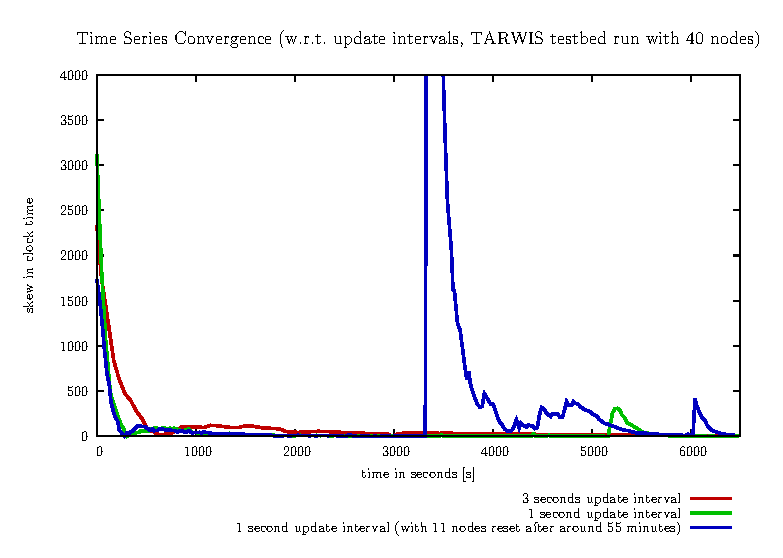
\includegraphics[scale=0.8]{images/FIG_02.eps}
	\caption{Time series convergence with respect to update intervals}
	\label{fig:update_intervals}
\end{figure}
\noindent On the other hand when we decrease the time synchronisation update interval, we can see that the assimilation of the nodes responds in an almost linear way to these changes, i. e. when we set the interval three times as high, the assimilation phase only takes roughly a third of the time. We visualise this in figure \ref{fig:update_intervals}. In addition, a spike can be identified where some nodes have been reset.\\

\begin{figure}[H]
	\centering
	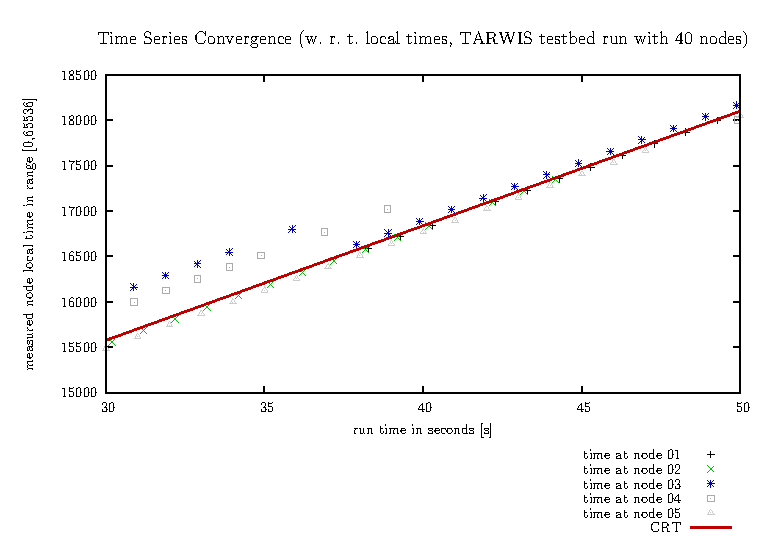
\includegraphics[scale=0.8]{images/FIG_03.eps}
	\caption{Time series convergence with respect to some node's local time}
	\label{fig:local_time}
\end{figure}

\noindent Next, we analyse the clock value over time. In figure \ref{fig:local_time} we see vertically each nodes current clock value at a specific point in time (x-axis). The gaps are representing the random wait of the node, before he starts the next RTT request cycle. The random wait is a result of introducing some randomness, because we want a guarantee that the nodes would not infer each other in a repetitive way. We see that all lines are slowly pointing towards a common center line, we call this the cluster reference time (CRT). This CRT can be determined for each single node with respect to the neighbours and it is perfectly diagonal in any plot per definition. In the end it is our goal to ensure as accurate as possible that the CRT is the same for all nodes. Please consider, that the plots only visualise a small fraction of the synchronisation process inside a specific node (hence, it represents even a smaller field in the whole sensor network).\\

\noindent Nevertheless, we were also interested in the discovery time of the neighbours. We saw in our experiments, that  in most cases all neighbours could be identified after 300 seconds. In some specific cases, this interval was much larger for some nodes. These nodes appear to have encountered a crowded channel, or poor signal strength in general.\\

\noindent For all runs we obtained a maximal accuracy around the value of alpha. This can easily be explained: The changes being made to each nodes clock are \code{[calculated\_mean\_skew * (1 / alpha)]} and the device doesn't contain a float\-ing-point unit (FPU), so the all skews smaller than 5 for an alpha set to 5 result in a skew change of 0.

\section{Conclusions}

We were able to implement the demanded work and the results are quite promising. Nevertheless, the accuracy and the convergence speed depend highly on the used parameters. We identified an alpha value around 1 to be the most robust solution, whereas the update interval should be defined as small as possible to ensure a quick convergence. However, if the interval was set too low, the TARWIS testbed crashed and wasn't able to respond anymore. In our experiments we found an update interval of one second to be the best trade-off between reliability and convergence speed. 

\bibliography{biblio}{}

%The bibliography, done here without a bib file
%This is the old BibTeX style for use with llncs.cls
\bibliographystyle{splncs}

%Alternative bibliography styles:
%the following does the same as above except with alphabetic sorting
%\bibliographystyle{splncs_srt}
%the following is the current LNCS BibTex with alphabetic sorting
%\bibliographystyle{splncs03}
%If you want to use a different BibTex style include [oribibl] in the document class line


\end{document}

